% ---------------------------------------------------------------------------
% Method panel: the pipeline, what "observable" means once time is involved,
% the algorithm steps, and validation.
% ---------------------------------------------------------------------------

% One stage of the pipeline band.  Chips are placed at explicit coordinates so
% the band reads right-to-left like the rest of the poster.
\newcommand{\StageChip}[4]{%
  \node[
    anchor=center,
    rounded corners=.26cm,
    fill=PosterPurple!#4,
    text=white,
    minimum width=7.05cm,
    minimum height=1.90cm,
    inner sep=.14cm
  ] (#1) at (#2)
    {\RTLnodebox{6.55cm}{\centering\fontsize{17}{21}\selectfont #3\par}};
}

\newcommand{\MethodContent}{%

ورودی، فایل \code{.statespace} افراست؛ بدون ویرایش دستی. کاربر \emph{مجموعهٔ
مشاهده} را می‌دهد و هر تعامل دیگری به گذار داخلی $\tau$ بدل می‌شود.

\vspace{.10cm}
\begin{center}
\begin{tikzpicture}[>=stealth,line width=1.2pt]
  % Row 1, read from the right.
  \StageChip{s1}{ 8.00,0}{خواندن خروجی افرا\\[-.10cm]{\footnotesize\code{.statespace}}}{100}
  \StageChip{s2}{ 0.00,0}{پنهان‌سازی تعامل‌های\\[-.10cm]خارج از مجموعهٔ مشاهده}{86}
  \StageChip{s3}{-8.00,0}{شکستن یال‌های زمانی\\[-.10cm]به گام‌های یک‌واحدی}{72}
  % Row 2, also read from the right.
  \StageChip{s4}{ 8.00,-2.72}{پالایش افراز\\[-.10cm]تا رسیدن به پایداری}{58}
  \StageChip{s5}{ 0.00,-2.72}{ساخت خارج‌قسمت و\\[-.10cm]فشرده‌سازی زنجیرهٔ زمان}{44}
  \node[
    anchor=center,rounded corners=.26cm,fill=PosterGreen,text=white,
    minimum width=7.05cm,minimum height=1.90cm,inner sep=.14cm
  ] (s6) at (-8.00,-2.72)
    {\RTLnodebox{6.55cm}{\centering\fontsize{17}{21}\selectfont
       وارسی مستقل\\[-.10cm]رابطهٔ خروجی و ورودی\par}};

  \draw[->,PosterPurple!70] (s1) -- (s2);
  \draw[->,PosterPurple!70] (s2) -- (s3);
  \draw[->,PosterPurple!70] (s3.south) -- ++(0,-.40) -- (8.00,-1.37) -- (s4.north);
  \draw[->,PosterPurple!70] (s4) -- (s5);
  \draw[->,PosterPurple!70] (s5) -- (s6);
\end{tikzpicture}
\end{center}

{\postertitlefont\fontsize{27}{34}\selectfont زمان از دید مشاهده‌گر بیرونی\par}
\vspace{-.06cm}

{\fontsize{19}{25}\selectfont یال سیاه \code{a} کنش قابل مشاهده است،
\code{tau} گذار داخلی، و یال‌های قرمز گذر زمان با مدت دقیق.\par}

\vspace{.10cm}
\begin{latin}
\centering
\begin{tabular}{@{}r@{\hspace{.40cm}}l@{}}
  \fontsize{18}{22}\selectfont\bfseries TTS 1 &
    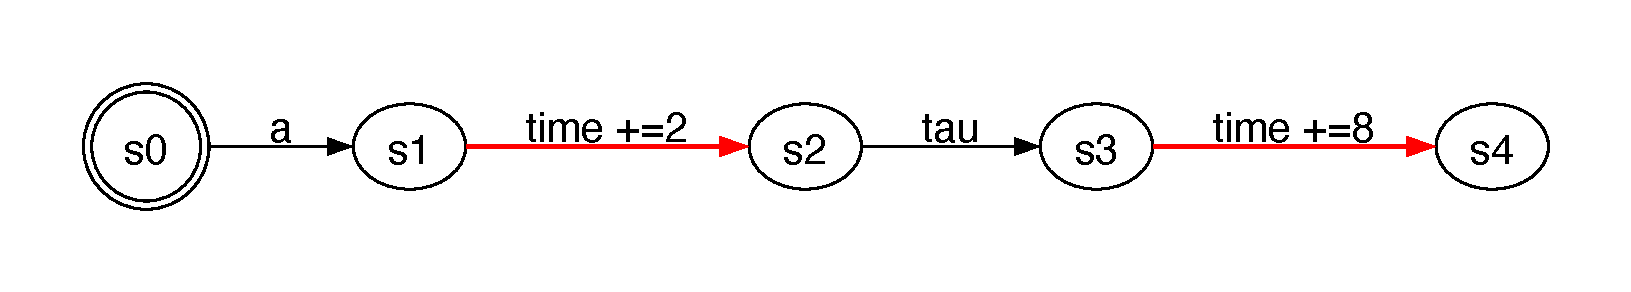
\includegraphics[height=2.00cm]{assets/figures/observable-then-split-delay.pdf}\\[.18cm]
  \fontsize{18}{22}\selectfont\bfseries TTS 2 &
    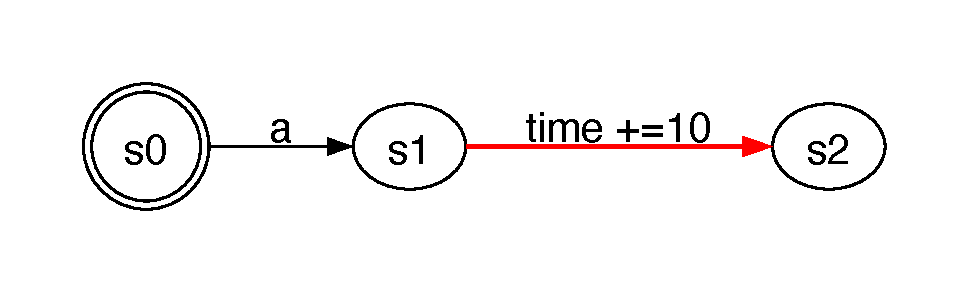
\includegraphics[height=2.00cm]{assets/figures/observable-then-delay.pdf}\\[.18cm]
  \fontsize{18}{22}\selectfont\bfseries TTS 3 &
    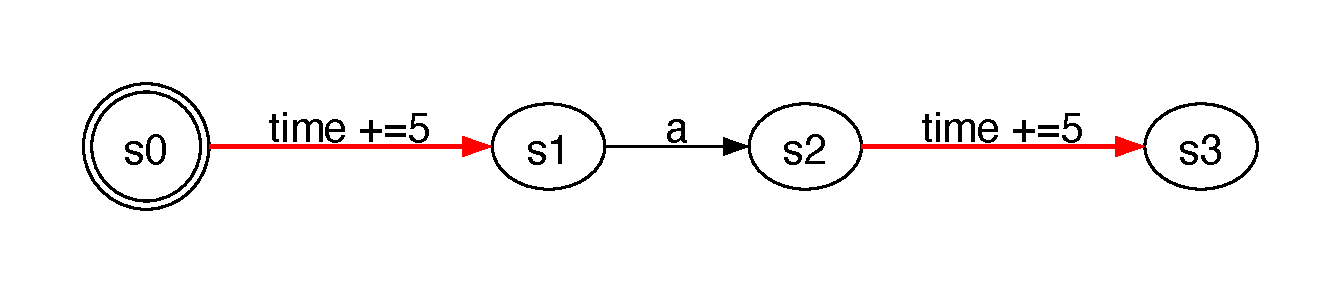
\includegraphics[height=2.00cm]{assets/figures/delay-observable-delay.pdf}\\
\end{tabular}
\end{latin}
\vspace{.14cm}

در \code{TTS 1} و \code{TTS 2} کنش \code{a} در لحظهٔ صفر رخ می‌دهد و سپس ده واحد
زمان می‌گذرد؛ گام داخلی \code{tau} دیده نمی‌شود و زمان سپری‌شده را از نو آغاز
نمی‌کند، پس این دو \textbf{هم‌ارزند}. در \code{TTS 3} هم ده واحد زمان می‌گذرد،
اما \code{a} پس از پنج واحد رخ می‌دهد: پنهان‌سازی روی گذارهای داخلی اعمال
می‌شود، نه روی \emph{لحظهٔ} وقوع یک کنش قابل مشاهده. پس \code{TTS 3} با آن دو
\textbf{هم‌ارز نیست}.

\vspace{.10cm}
{\fontsize{20}{26}\selectfont
\PosterLead{گام‌های الگوریتم ---}\par
\PosterLead{۱.} هر یال زمانی با مدت $d$ به $d$ یال یک‌واحدی شکسته می‌شود؛
حالت‌های میانیِ تازه شناسه‌های یکتا می‌گیرند تا با حالت‌های موجود اشتباه نشوند.\par
\PosterLead{۲.} حالا همهٔ گذارهای زمانی برچسب یکسان \code{delay(1)} دارند، پس
پالایش افراز زمان و کنش را یکنواخت بررسی می‌کند، بی‌آنکه روی مقدار $d$ کرانی
لازم باشد.\par
\PosterLead{۳.} افراز تا پایداری پالایش می‌شود؛ سپس خارج‌قسمت ساخته و
زنجیره‌های صرفاً زمانی در یک یال با مدت جمع‌شده فشرده می‌شوند.\par
\vspace{.12cm}
\vspace{.10cm}
\PosterLead{ابزار:} \code{awtr} — جاوا ۱۷؛ فرمان‌های \code{reduce}،
\code{equivalent}، \code{inspect} و \code{visualize}. خروجی اصلی
\code{reduced.json} است، در کنار \code{partition.json} که هر حالت ورودی را به
ردهٔ خود نگاشت می‌کند. توسعه آزمون‌محور (\code{TDD}) پیش رفت: ۱۱۶ آزمون واحد و
۶۲ بررسی انتهابه‌انتها.\par}

\PosterHighlight[PosterGreen]{%
کاهش‌دهنده و وارسی‌گر دو مسیر کد \emph{جداگانه}‌اند: وارسی‌گر رابطهٔ خروجی و
ورودی را مستقل از الگوریتم کاهش بازمی‌سنجد.}
}
